 \section{Disclaimer}\index{Disclaimer}

Einstein's theory of special relativity is one of the most fascinating, elegant, surprising, and powerful theories in modern physics.  The derivation of its laws, beginning from the simple postulate that the speed of light is a constant, independent of the velocity of the person measuring it, along with the resulting profound implications in electromagnetic theory and the nature of space and time is astounding. We, unfortunately, do not have the time to cover everything in this course.  And you, as freshmen, for the most part are just not ready.  You will study this theory in depth when you take 300-level E\&M.

However, to understand what is going on at the LHC, you do need to understand some relativity.  The goal of this tutorial is to teach you the minimum needed to understand the Higgs discovery.  We will approach it from a practical point of view. Although this is anathema to the physicist in you, we will give you formulas without telling you where they come from.  You need to just accept them (For now! Until you are older!) as experimental reality, just as you accept $\vec{F}=m\vec{a}$  as a fact that you can use as a tool to work other problems.

\section{4-vectors}\index{4-vectors}

When doing Newtonian mechanics, you are taught about vectors.  You typically work with vectors that have three components, associated with three spatial directions (x, y, z).  Often, you then parameterize these components as a function of a time.  You might calculate the height of a particle above the ground (z) as a function of time, its z-component of velocity as a function of time, or its momentum as a function of time.

With special relativity, instead of these 3-vectors, we will work with 4 component vectors (4-vectors).  The fourth component for our position vector will be {\it time}.  However, time and position have different units (seconds for time and meters distance).  Mixing time and distance is thus mixing apples and oranges, so what can be done?

In special relativity, the speed of light is very special.  It is a constant, and all observers, regardless of their relative velocity, will get the same result when they measure it. We will discuss this more later.  Since this is a special number, one of the {\it fundamental constants} of nature, along with  $\hbar$ the fundamental constant of quantum physics, and a few other fundamental numbers.  We can use c to convert time to a distance and write our 4 vector for {\it event} (something that has a time and a position) as
\begin{equation}
	  {\color{red} d}=(ct,x,y,z)
\end{equation}

\noindent Every 3-vector will be augmented this way, although the associated {\it time-like component} may not be obvious to you at this stage.  Most importantly, momentum becomes 4-momentum, defined as
\begin{equation}  
{\color{red} p}=(E,cp_x, cp_y, cp_z)  
\end{equation}

where E is the particle's energy. Again, we use c to make sure all components have the same units.
	 
We will use red to denote 4 vectors and the usual vector notation to denote 3 vectors.  Thus we can write:
\begin{equation} 
\textcolor{red}{p}=(E,cp_x, cp_y, cp_z)  
\end{equation}  		   
\begin{equation} 
{\color{red} p}=(E,c\vec{p})  
\end{equation} 
\vspace{.2cm} 
\begin{minipage}{0.9\textwidth} 
\begin{framed}
%\vspace{.1cm}
\begin{exercise}
%\begin{frshaded}
%\fcolorbox{\bordercolor}{\backgroundcolor} 
{show that E and cp have the same units. Remember that the $i^{th}$ component of force is related to energy by $F_i=\frac{dE}{dx_i}$
 and to momentum by $F_i = \frac{dp_i}{dt}$}
\end{exercise}
%\end{frshaded}
%\vspace{.1cm}
\end{framed} 
\end{minipage}
\vspace{.2cm}



As you may remember from your high school physics, there are several important mathematical operations that are used with vectors.  One is the dot product, a way of making a scalar out of two vectors.  You may remember that:
\begin{equation}
      C= \vec A \cdot \vec B = A_xB_x +A_yB_y +A_zB_z 
\end{equation}
The dot product of a vector with itself gives the square of the magnitude of the vector.
\begin{equation}      
     |{\vec{A}|^2} =\vec A \cdot \vec A  
\end{equation}	  
\noindent The dot product, in Newtonian physics, is used in calculating work from force and displacement.

There is a dot-like product associated with 4 vectors, and it has some very interesting, useful, and sometimes bewildering properties.
\begin{equation}
	    c ={\color{red}a} \cdot {\color{red}b} = a_0b_0 - \vec a \cdot \vec b
\end{equation}
More on this useful operation later.

\section{Frames (center-of-mass, lab) and transforming between frames}\index{Frames (center-of-mass, lab) and transforming between frames}

Imagine two people, (A and B) with rulers and stop watches.  A is standing in the sidewalk on Route One, while B is in a white car in the left hand lane going south on Route One.  Both see a red car in the right hand lane going south which passes the car containing B.  However, person A sees the space between her and red car increasing at a much faster rate than person B sees the space between him and the red car increasing.  They each measure a different velocity for the red car relative to themselves.  Mathematically, what we have in 1 spatial dimension; it is easy to extend to 3 spatial dimensions.

\noindent let $v_B, x_B$ be the velocity and relative to person A 
       
\noindent let $v_{RA}, x_{RA},v_{RB}, x_{RB}$
	  

Then,
\begin{equation}
 v_{RB} = v_{RA} - v_B
\end{equation}
\begin{equation}
 x_{RB} = x_{RA} - v_B t
\end{equation}

\noindent This set of equations that transform a variable as it is measured in one frame to the value it will have when measured in another frame is called {\it Galilean Relativity}.


However, in relativity, if the red car were moving at the speed of light both A and B would see the distance between them and the car increasing at the same rate.  In other words, all observers will measure the same speed of light regardless of their relative velocities.  Obviously, the equations given above do not predict this.  Einstein developed new equations that give us a measurement in one frame relative to another.  


\begin{equation} ct_{RB} = \gamma(ct_{RA} - \beta x_{RA}) \end{equation} 
\begin{equation}  x_{RB} = \gamma(- \beta ct_{RA} + x_{RA}) 	 \end{equation} 

\noindent where,

\begin{equation} \beta = v_B /c \end{equation}   	
\begin{equation} \gamma = \frac{1}{\sqrt{1- \beta^2}} \end{equation}  


Note that $\beta$  is a number between 0 and 1, and is the fraction of the speed of light the other measured frame has with respect to your frame of reference.  $\gamma$  is a number that is greater than 1.  It is called the {\it relativistic boost} and will be very useful.

In general, any 4-vector will transform this way.  Thus, the energy-momentum 4-vector will transform in this way.  This set of transformation equations is called {\it Special Relativity} or the {\it Lorentz transformation}.

Note that these are extremely weird equations.  They imply that observers that are not at rest with respect to each other will not agree on the time when something occurred. They will not agree if two things happening at two different positions happened at the same time or not.  There are lots of fascinating implications to this, but you will just have to take more advanced physics to learn about them.  We are going to concentrate on the minimum you need to look for new particles at the LHC.

\section{Length of 4 vectors}\index{Length of 4 vectors}

A 4 vector has the interesting property that all observers, regardless of their relative velocities, will agree on: the length of a 4-vector.
Let's prove this in one spatial dimension (I think you can do the
equivalent proof in 3-D using this model!). 

Lengths of 4 vectors
\begin{eqnarray}
|a|^2 &=&  a_0 a_0 - a_x a_x  \nonumber \\
      &=&  |a'|^2 = a'_0 a'_0 - a'_x a'_x  \nonumber \\
      &=& \gamma (a_0 -\beta a_x) \gamma (a_0 -\beta a_x) - \gamma (-\beta a_0 +a_x ) \gamma (-\beta a_0 +a_x )  \nonumber \\
      &=&  \gamma^2 (a_0^2  -2 \beta a_x a_0  + \beta^2 a_x^2 - \beta^2 a_0^2  + 2 a_x \beta  a_0  - a_x^2)   \nonumber \\
      &=& =\gamma^2 ( a_0^2 (1-  \beta^2)  - a_x^2 (1-  \beta^2))   \nonumber \\
      &=&  a_0^2 - a_x^2  \nonumber  \\
      &=& |a|^2  
\end{eqnarray} 

In particular, this is true for the energy-momentum 4 vector  $|{\color{red}p}|^2 = E^2 - (pc)^2$  . (working in 1 spatial dimension! you can extend this to 3)  In fact, 
\begin{equation}
	  	(mc^2)^2 = E^2 -(pc)^2
\end{equation}  
In the rest frame of a particle (the frame where  $|\vec p |$  is zero), you get the famous equation that appears on T-shirts everywhere.

This equation is very important to the LHC.  When we look for particles, we recognize them by their mass.  W bosons have a mass of 80 GeV.  Z bosons have a mass of 91 GeV.  Top quarks have a mass of 173 GeV.  Obviously, we cannot put particles on a scale to weigh them. This equation tells us that, if we want to see the mass of a particle made in a collision, we just need to know its energy and momentum.  Then, from that, we can determine its mass.  We can also show that it doesn't matter what our velocity is with respect to the particle.  This equation will always give us the mass of that particle, and that all observers will agree on the mass.

\section{HEP units}\index{HEP units}

Masses in GeV?  What kind of mass unit is that? You may be more used to kg or g or lbs.  Remember that the eV is a unit of energy, defined as the potential energy gained when an electron moves from one position to another whose potential is higher by 1 V.

We know from Einstein that mass is related to energy through $c^2$.  So $eV/c^2$ is a unit of mass.  GeV/$c^2$ is then $10^6$ eV/$c^2$.  For scale, the proton has a mass of 1 GeV/$c^2$.

Particle physicists are lazy.  They hate to type even a single extra letter.  Particle physicists are lazier than most.  They have defined a whole unit system designed to help them avoid typing $c$ and $\hbar$ .  Unit systems need a way of defining a time unit, a distance unit, and a weight unit.  

$c$ is related to both the time and distance unit.  The units of  $\hbar$ are Energy x time. We know from Einstein that energy is related to mass, so we can use it instead of mass as our third necessary unit.  The eV, which is the potential energy an electron gains when it transverses a potential difference of 1 V, is chosen to be the unit of energy. Length and time units are then chosen so that both $c$ and $\hbar$  are 1.  

Once we do that, GeV/$c^2$ just becomes GeV/$1^2$ or GeV. Not only that, but we can also measure both length and time in GeV.

\noindent For example  $\hbar$/GeV is a unit of time.  But $\hbar$ =1 in this unit system, so GeV$^{-1}$ is a unit of time.  c/GeV is a unit of length.  So GeV$^{-1}$ is also a unit of length.


In this unit system, the length of the energy-momentum 4-vector becomes (in 1 dimension):
\begin{equation}
	  m^2 = E^2 - p^2
\end{equation}  	 


\section{Lifetimes of particles}

An interesting consequence of special relativity is that the lifetime you measure for a particle will depend on its velocity relative to you.  Let $\tau _0$  be the lifetime you measure for the particle when the particle is at rest with respect to you.  Then, using equation 1.4, we can see that the lifetime for a particle moving with a velocity $\beta$  is
\begin{equation}
	 \tau  = \gamma \tau _0
\end{equation}  	 

\noindent The lifetime is longer for a moving particle than it is for one at rest by a factor $\gamma$.

\section{Breit-Wigner}

We have learned that most heavy particles are not stable, and decay.  Above, we said that particles are identified by their mass, and that particles have a well-defined mass characteristic of their type.  However, this is not quite true.  As you will learn when you take quantum mechanics, a quantum state cannot have a well defined time and a well defined energy (mass).  This is expressed through the Heisenberg uncertainty principle:
\begin{equation}
	 \Delta E \Delta t   \ge \hbar
\end{equation} 

\noindent Because of this, when we measure the particle's mass, we get a range of values.  How big is that range?  Remember that we can express the lifetime of a particle, using our new funny units, in GeV, using:
 \begin{equation}
	 \Gamma =   \frac{\hbar}{\tau _0}
\end{equation} 
	  

\noindent where  $\Gamma$ is the lifetime in GeV.  When the lifetime is expressed in GeV,  it is referred to as the particle's width.

\noindent The actual functional form of the mass distribution is called a Breit-Wigner.  The form is:

\begin{equation} \text{rate  of  events} \propto \frac{1}{(E-M)^2 + \frac{\Gamma}{2}} \end{equation} 

\noindent where M is the value of the peak of the mass distribution and E is the observed mass.

\vspace{.2cm} 
\begin{minipage}{0.9\textwidth} 
\begin{framed}
%\vspace{.1cm}
\begin{exercise}
%\begin{frshaded}
%\fcolorbox{\bordercolor}{\backgroundcolor} 
{For the Z boson, M is 91.2 GeV and $\Gamma$  is 2.5 GeV.  What is the corresponding lifetime?  Use root to plot this function versus E, the observed mass.}
\end{exercise}
%\end{frshaded}
%\vspace{.1cm}
\end{framed} 
\end{minipage}
\vspace{.2cm}



\section{The coordinate system for a collider experiment}

The CMS detector, whose data we will be using in this course, uses a right-handed coordinate system, with the origin at the nominal interaction point, the x axis pointed to the center of the LHC, the y axis pointing up (perpendicular to the LHC plane), and the z axis along the anticlockwise-beam direction.  The polar angle   is measured from the positive z axis and the azimuthal angle  $\phi$  is measured in the x-y plane.

\section{Collisions (conservation of 4-momentum)}

When two protons appear to collide in a detector, what really collides is the {\it partons} (either quarks or gluons) inside the protons.  A sketch of a collision that produces a Z boson is shown below.
 

\begin{figure}[h]
\centering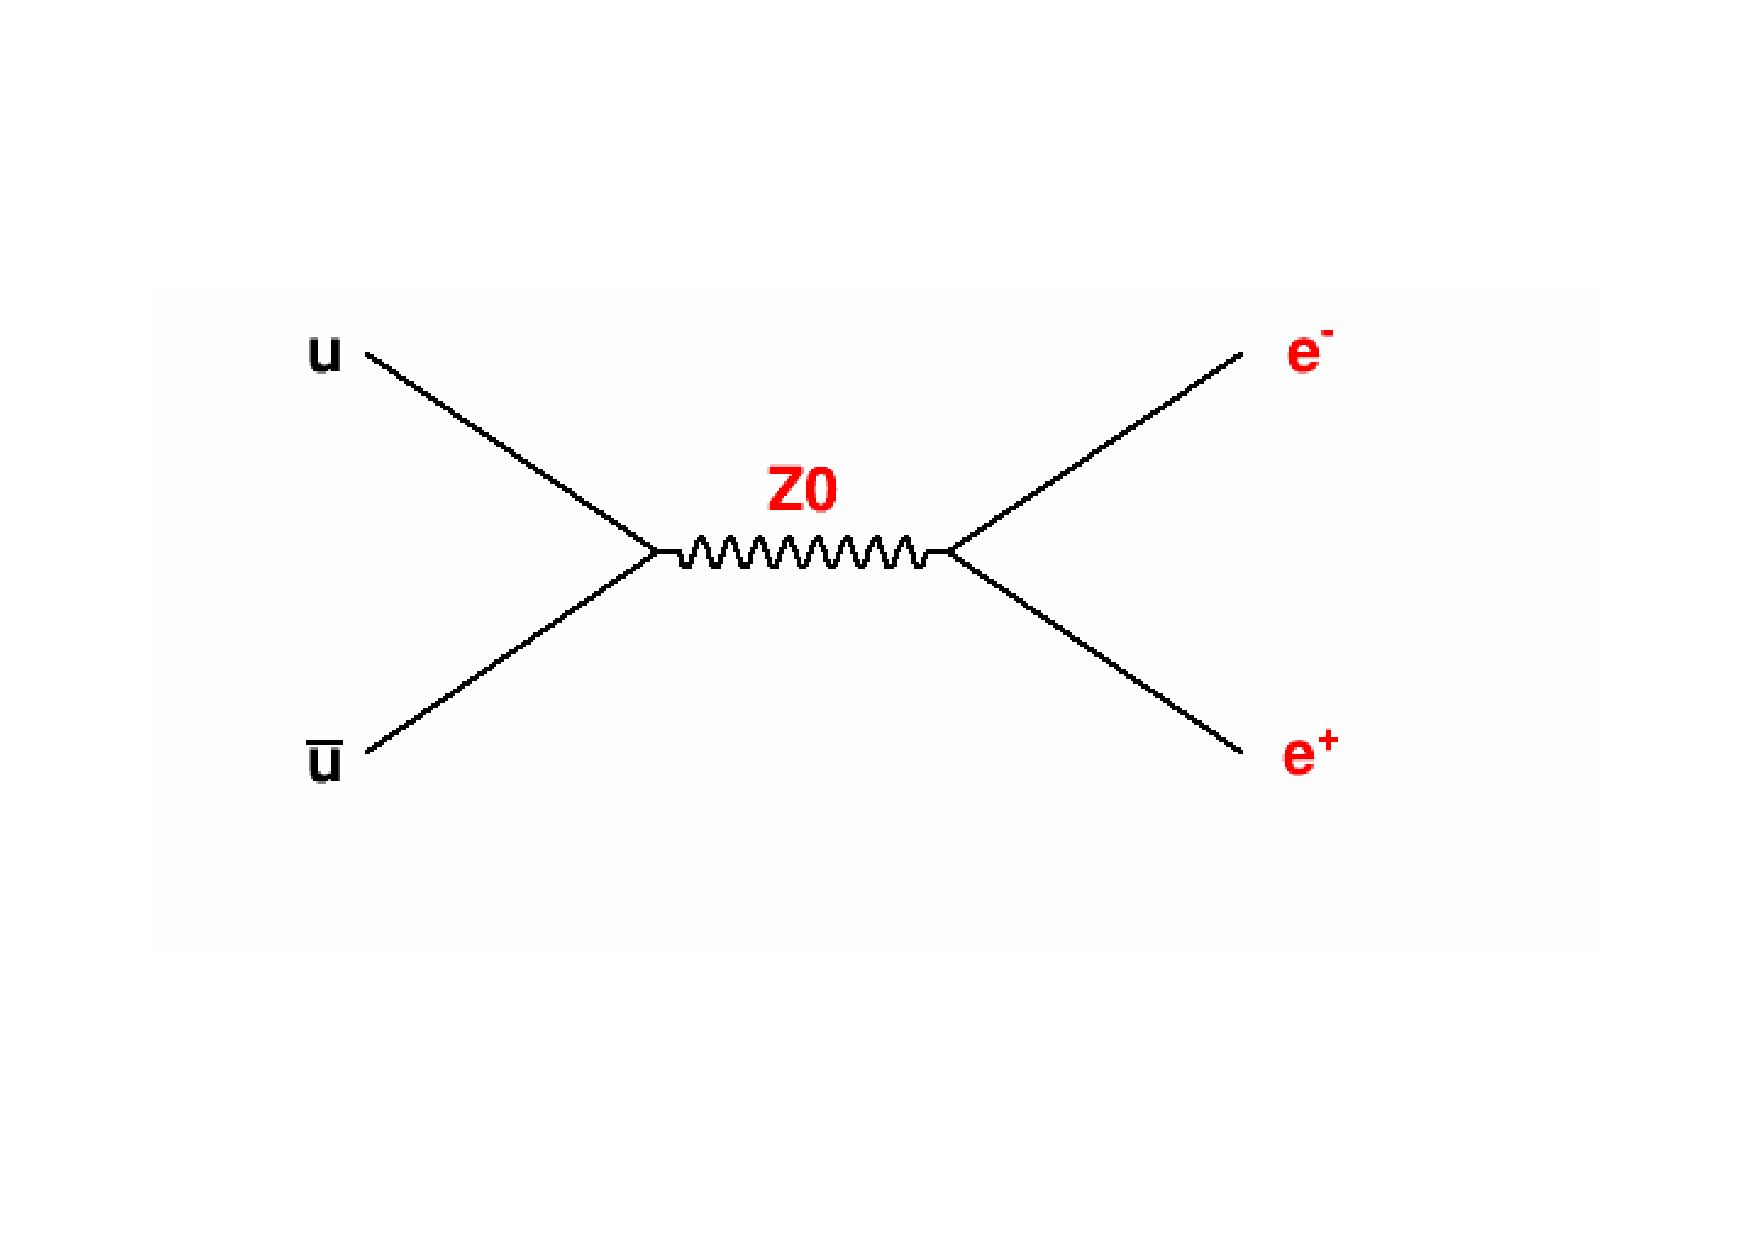
\includegraphics[scale=0.4]{./relativity/Pictures/FeynmannDiagram.pdf}
\caption{Feynman diagram for production of a Z boson in a proton-proton collision, with subsequent decay to electrons}
\label{fig:collrel}
\end{figure}




The total momentum of the proton is divided among the partons in an unequal way that varies collision by collision.  Sometimes most of the momentum is held by a single parton.  Sometimes it is divided among a very large number of partons.  We can know the distribution of probabilities versus fraction of proton momenta, but cannot know, for a specific collision, what fractions the colliding partons had.  It will be very rare, however, for both partons to have equal but opposite momenta in the lab frame.

It is usually easiest to understand this collision if we transform to the frame where the partons do have equal but opposite momenta.  This special frame is called the center-of-mass frame.  In this frame, the partons have equal but opposite 3-momenta.  The total initial state 2-momenta, therefore, is zero.  Since momentum is conserved, this means the Z boson produced must have zero 3-momenta and therefore zero kinetic energy.  Its only energy will be that due to its mass.  Since energy is also conserved, this means the initial energies of the partons must be half the Z mass (ignoring for now the finite width of the Z).  Since the partons are approximately massless, this means that the initial momenta of the partons must be:

\begin{equation}
 p_{u} = ( {M_z \over 2},0,0,{M_z \over 2})
\end{equation}
\begin{equation}
 p_{\bar{u}} = ( {M_z \over 2},0,0,-{M_z \over 2})
\end{equation}

\noindent What about the electrons that are produced?  Again, due to conservation of momentum, their 3-momenta must be equal and opposite.  And, from conservation of energy, their energies must be half the Z mass.  Because they are approximately massless, the magnitude of their 3-momenta must be equal to their energy.  However, their 3 momenta do not have to be along the z axis.  So, in general:

\begin{equation}
 p_{e^+} = (\frac{M_Z}{2}, \frac{M_Z}{2} cos \theta cos \phi ,  \frac{M_Z}{2} cos \theta sin \phi , \frac{M_Z}{2} sin \theta) 
\end{equation}
\begin{equation}
 p_{e^-} = (\frac{M_Z}{2}, \frac{M_Z}{2} cos (\pi - \theta) cos \phi ,  \frac{M_Z}{2} cos  (\pi - \theta) sin \phi , \frac{M_Z}{2} sin  (\pi - \theta)) 
\end{equation}


	  
The probability distribution for the polar and azimuthal angles are predicted by the standard model, but is beyond the level of this course.

What will this look like in the lab frame?

Since to boost back into the lab frame, we do a boost along the z axis, only the z components of 3-momentum will change.  The x and y components will stay the same.  The energy will change as well, since (in the massless, highly relativistic approximation)
\begin{equation}
E^2 = p_x^2 + p_y^2 + p_z^2   
\end{equation}
The polar angle changes, but the azimuthal angle does not.  Because of this, transverse variables are very important to collider physicists; they are most sensitive to the particle produced, and not sensitive to the boost.

The component of momentum transverse to the beam axis is called the {\it transverse momentum}.  It's magnitude is calculated:
\begin{equation}
	 p_T =   \sqrt{p_x^2 +p_y^2}
\end{equation} 
  

You will see this variable over and over when you work on hadron collider physics.

\section{Rapidity and Pseudorapidity}

Another variable related to boosts and the polar angle is the rapidity, defined as:

\begin{equation}
	 y =  \frac{1}{2} ln (\frac{E + p_z}{E-p_z})
\end{equation} 
	  

\vspace{.2cm} 
\begin{minipage}{0.9\textwidth} 
\begin{framed}
%\vspace{.1cm}
\begin{exercise}
%\begin{frshaded}
%\fcolorbox{\bordercolor}{\backgroundcolor} 
{show that the difference in rapidity between two particles is independent of the boost in the z direction.}
\end{exercise}
%\end{frshaded}
%\vspace{.1cm}
\end{framed} 
\end{minipage}
\vspace{.2cm}




A related variable is the pseudorapidity, defined as:

\begin{equation}
	 \eta  = - \ln{\tan{\frac{\theta}{2}}}
\end{equation} 


\vspace{.2cm} 
\begin{minipage}{0.9\textwidth} 
\begin{framed}
%\vspace{.1cm}
\begin{exercise}
%\begin{frshaded}
%\fcolorbox{\bordercolor}{\backgroundcolor} 
{show that rapidity and pseudorapidity are equal for massless particles.}
\end{exercise}
%\end{frshaded}
%\vspace{.1cm}
\end{framed} 
\end{minipage}
\vspace{.2cm}



\section{Further reading}
\begin{itemize}	
\item http://en.wikibooks.org/wiki/Special\_Relativity
\end{itemize}

